\parindent=0em
\subsection{Teléfonos móviles}
\label{sec:telefonosMoviles}
\noindent

%https://www.aniwaa.com/product/vr-ar/tesseract-holoboard-enterprise-edition/

Los teléfonos móviles son un gran dispositivo ya que combinan GPS, cámara, brújula y un acelerómetro, cubriendo así las necesidades de una aplicación de realidad aumentada~\cite{arsmartphones}, además, es un dispositivo muy común entre la población lo cual facilita el desarrollo y expansión de esta realidad. Por otro lado, los teléfonos móviles se pueden utilizar también para realidad mixta utilizando unos cascos en los que se introduce el dispositivo para generar una experiencia de MR.\\

Existen distintos HMD que se utilizan para estas experiencias de realidad mixta acoplando los móviles a alguna parte de las gafas, como por ejemplo, las \textit{Holoboard Enterprise Edition} de la mano de la empresa \textit{TESSERACT} (figura~\ref{fig:mrandroidTESSERACT}). Este dispositivo es compatible a partir de Android 6.0  y como especificaciones técnicas se pueden destacar sus 82\degree~ de FOV, utiliza la tecnología SLAM para el \textit{tracking}, posee un controlador 6DoF y utiliza el \textit{tracking} por sensores IMU, además, permite experiencias colaborativas en la nube.

\begin{figure}[H]
    \centering
    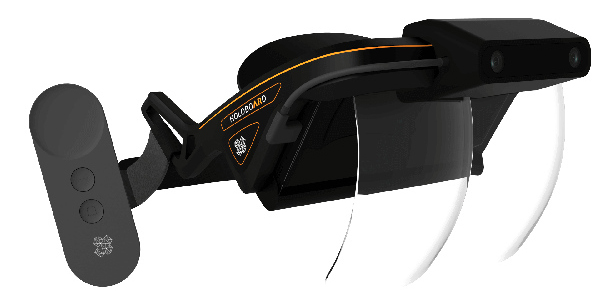
\includegraphics[scale=0.3]{Images/Estado del arte/mrandroid.jpg}
    \caption[\textit{Holoboard Enterprise Edition}]{
    \textit{Holoboard Enterprise Edition\footnotemark.}
    }
    \label{fig:mrandroidTESSERACT}
\end{figure}
\footnotetext{Fuente: \url{https://www.aniwaa.com/product/vr-ar/tesseract-holoboard-enterprise-edition}}
En cambio, si estamos hablando de un dispositivo para utilizar en móviles con iOS podemos hablar del casco \textit{Bridge} (figura~\ref{fig:mriosBRIDGE}) de la empresa \textit{Occipital}. Este HMD requiere de un componente extra llamado \textit{Occipital Structure Sensor}, el cual, se utiliza para el escaneo 3D del entorno.

\begin{figure}[H]
    \centering
    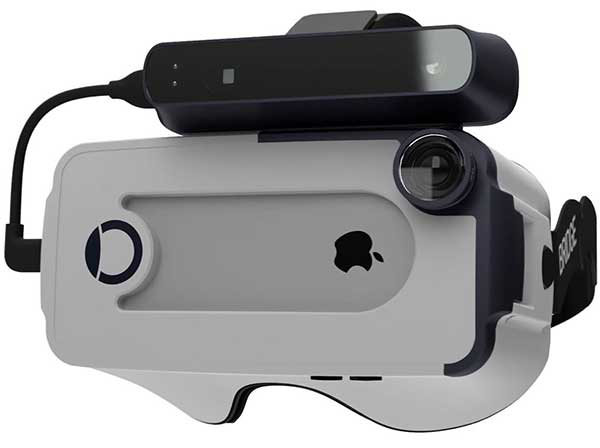
\includegraphics[scale=0.3]{Images/Estado del arte/mrios.jpg}
    \caption[\textit{Occipital Bridge}]{\textit{Occipital Bridge\footnotemark.}}
    \label{fig:mriosBRIDGE}
\end{figure}

\footnotetext{Fuente: \url{https://www.aniwaa.com/product/vr-headsets/occipital-bridge/}}

Las gafas \textit{Bridge} tienen un FOV de 120º, un controlador de 6DoF y destacan por que gracias a estas se puede utilizar aplicaciones de realidad aumentada, realidad mixta y realidad virtual, también, utiliza la técnica de \textit{tracking} conocida como \textit{inside-out}.\\

Pese a que la principal diferencia entre las dos gafas es el sistema operativo para el que están destinadas, se puede observar que los precios son similares y que las gafas destinadas para iOS poseen un FOV notablemente superior.


\begin{table}[H]
\centering
\renewcommand{\arraystretch}{1.5}
\begin{tabular}{llllll}
\toprule
Dispositivo                  & Precio & DoF & FOV & \textit{SO} & \textit{Tracking} \\
\midrule
\textit{Holoboard Enterprise Edition} & \$399  & 6DoF         & 82\degree           & Android     & SLAM              \\
\textit{Occipital Bridge }            & \$349  & 6DoF         & 120\degree          & iOS         & \textit{Inside-out}\\\bottomrule       
\end{tabular}
\caption{Comparación entre ambas gafas de \textit{MR} para móviles.}
\label{cuadro:comparacionphonesMR}
\end{table}

